\documentclass[journal]{IEEEtrancz}
% zvolte kodovani
\usepackage[utf8]{inputenc} % linux/unix
%\usepackage[latin2]{inputenc}
%\usepackage[cp1250]{inputenc} % Windows
\usepackage[czech]{babel}
\usepackage{graphicx}

\begin{document}

\title{Semestrální práce předmětu a0m33eoa - TSP s několika cestujícími}
\author{Jakub Moravec}

\maketitle

\begin{abstrakt}
V práci jsou popsány tři algoritmy pro řešení problému TSP s několika cestujícími - lokální prohledávání, evoluční a memetický algoritmus. 
Ty jsou následně porovnány na třech různých datasetech a výsledky porovnány. 
\end{abstrakt}

\IEEEpeerreviewmaketitle

\section{Zadání}
Úkolem je vyřešit úlohu TSP s několika cestujícími pomocí heuristických algoritmů. Na vstupu je úplný neorientovaný graf o \textit{N} uzlech. Cílem je nalézt takovou množinu cest pro \textit{M} cestujících, které všechny vychází z počátečního uzlu (depotu) a zase v něm končí, všechny uzly (kromě depotu) jsou navštíveny právě jednou a délka nejdelší cesty je minimální. Žádná z cest nesmí mít nulovou délku.

\section{Úvod}
Úloha TSP s několika cestujícími známá také jako \textbf{VRP} (\textit{Vehicle routing problem}) je kombinatorická optimalizační úloha odpovídající otázku "Jaké je optimální uspořádání hran pro několik cestujicích tak, aby byly výsledné cesty pokrývající všechny uzly nejkratší?". Určení optimálního řešení tohoto problému je \textit{NP-těžká} úloha, proto bývá částo řešena pomocí heuristik a aproximačních algoritmů. V tomto dokumentu budou představena řešení pomocí \textit{lokálního prohledávání}, \textit{evolučního algoritmu} a \textit{memetického algoritmu} (kombinace předcházejících). 

% fitness fce
\textit{Fiteness funkce} pro vyhodnocování optimality řešení byla převzata ze zadání úlohy: kvalita řešení je určena jako délka nejdelší cesty z M cest. Tuto fitness funkci se budeme snažit minimalizovat. Délka cesty je určena \textit{Euklidovskou vzdáleností} měst.

% reprezentace
Jako reprezentace řešení problému byla zvolena uspořádaná množnina identifikátorů měst, kde pořadí měst určuje pořadí jejich průchodu. Depot (id 0) je v množině obsažen \textit{M +1} krát, všechna ostatní města právě jednou. Tato reprezentace byla zvolena proto, aby bylo možné stejným způsobem použitými algoritmy měnit pořadí měst v cestách jednotlivých cestovatelů i přesouvat města mezi cestovateli.\footnote{Pro \textit{lokální prohledávání} byla zvolena jiná reprezentace (popsaná v odstavci \ref{sec:local-search}). Ta byla pro \textit{evoluční a memetický algoritmus} upravena do této podoby, protože ta je pro uvedené algoritmy vhodnější.} Příklad reprezentace úlohy s dvěmi cestovateli:

$$[0,1,3,5,7,0,9,2,4,6,8,0]$$ 

\section{Cíl práce}
Cílem práce je implementovat \textit{algoritmus lokálního prohledávání}, \textit{evolučníh algoritmus} a \textit{memetický algoritmus} generující řešení problému taková, aby jejich hodnota fitness funkce byla minimální a to při co možná nejmenším počtu vyhodnocení definované fitness funkce. 

%TODO
\section{Experimenty}
V této sekci budou představeny všechny implementované algoritmy, provedené experimenty a jejich výsledky. 

\subsection{Popis algoritmů}
\bigskip
\subsubsection{Lokální prohledávání}
\label{sec:local-search}
Reprezentace řešení pro tuto úlohu úlohu je odlišné, než u ostatních úloh. Řešení je reprezentováno dvěmi uspořádanými množinami, kde první určuje pořadí měst (neobsahuje depot), druhá obsahuje tzv. \textit{breakpointy}, které definují, kdy je ukončena cesta jednoho cestovatele a kam má tedy být vložen depot. Příklad reprezentace úlohy s dvěmi cestovateli:

$$[1,3,5,7,9,2,4,6,8][4]$$

Jako iniciální řešení jsou přebrána města v pořadí na vstupu a \textit{breakpointy} jsou rovnoměrně vygenerovány dle počtu cestovatelů.\footnote{To bylo při odevzdání bodově penalizováno, protože generování iniciálního řešení je deterministické a neobsahuje žádné náhodné prvky.}

Pro lokální prohledávání je implementován pertubační algoritmus vybírající nejlepšího jedince z \textit{k} vygenerovaných sousedů stávajícího řešení (\textit{best neighbour}). Pertubační operátor generuje okolní řešení prohazováním náhodných měst a náhodným posouváním \textit{breakpointů} o jednu pozici. Parametry algoritmu jsou uvedeny v tabulce \ref{tab:local-search}. Parametry byly určeny empiricky podle průběžných výsledků algoritmu.

\begin{table}
  \centering
  \caption{Parametry lokálního prohledávání}
  \begin{tabular}{|l||c|c|c|}
  \hline
  Počet sousedů  & 5 \\
  \hline
  Pravděpodobnost prohození měst  & 0.5 \\
  \hline
  Pravděpodobnost posunu \textit{breakpointu}  & 0.5 \\
  \hline
  \end{tabular}
  \label{tab:local-search}
\end{table}

\bigskip
\subsubsection{Evoluční algoritmus}
\label{sec:ea}
Evouční algoritmus používá následující operátory: 
\begin{itemize}
  \item{\textbf{Inicializace}}: První generace je inicializována zcela náhodnými řešeními. Každý jedinec je generován ze vstupních dat přidáním stejného počtu pivotů, jako je počet cestovatelů (jeden už je přítomen) a náhodným proházením pořadí měst.
  \item{\textbf{Křížení}}: Jako operátor křížení byl zvolen tzv. \textit{ordered crossover}, který vybere náhodnou sekvenci měst jednoho z rodičů, ty vloží do potomka a doplní je o zbylá města v pořadí dle druhého rodiče. Tento algoritmus byl upraven tak, aby zachovával počet pivotů v řešení.
  \item{\textbf{Mutace}}: Jako mutace je použit algoritmus náhodně prohazující dvě města v rámci celého řešení (tedy i mezi různými cestovateli).
  \item{\textbf{Selekce}}: Vzhledem k tomu, že definovaná fitness funkce je minimalizována, byla pro výběr jedinců do nové generace zvolena \textit{turnajová selekce}.
\end{itemize}  

Parametry evolučního algoritmu jsou uvedeny v tabulce \ref{tab:ea}. Parametry byly určeny empiricky podle průběžných výsledků algoritmu.

\begin{table}
  \centering
  \caption{Parametry evolučního algoritmu}
  \begin{tabular}{|l||c|c|c|}
  \hline
   Velikost populace  & 500 \\
  \hline
   Pravděpodobnost křížení & 0.6 \\
  \hline
   Pravděpodobnost mutace & 0.005 \\
  \hline
   Počet účastníků turnaje & 10 \\
  \hline
   Počet jedinců zachovaných do příští generace & 100 \\
  \hline
  \end{tabular}
  \label{tab:ea}
\end{table}

\bigskip
\subsubsection{Memetický algoritmus}
Memetický algoritmus kombinuje evoluční algoritmus a lokální prohledávání. Využívá následující operátory: 
\begin{itemize}
  \item{\textbf{Inicializace}}: Stejné jako u evolučního algoritmu (odstavec \ref{sec:ea}).
  \item{\textbf{Křížení}}: Stejné jako u evolučního algoritmu (odstavec \ref{sec:ea}).
  \item{\textbf{Mutace}}: Pro memetický algoritmus byla upravena mutace, ta náhodně vybere začátek či konec cesty (o náhodné délce) některého cestovatele a prohodí ho se začátkem či koncem cesty (o náhodné délce) jiného cestovatele. K této mutaci bylo přistoupeno proto, že na vygenerovaných řešeních bylo často patrné, že jsou vygenerovány špatně právě začátky a konce cest (cesty se proto často křížili apod.). Přidaná fáze lokálního prohledávání potom zaručí, že pokud takové prohození hodně "zpřehází" cesty, budou "narovnány".   
  \item{\textbf{Lokální prohledávání}}: Lokální prohledávání bylo přidáno jako samostatná fáze algoritmu, která je spouštěna po křížení a mutaci nad nově vygenerovanými řešeními. Jako algoritmus lokálního prohledávání byl zvolen \textit{2-opt} algoritmus. 
  Ten je spouštěn dvěmi různými způsoby, buďto pouze na cestě jednoho cestovate (změna neovlivní cesty ostatních cestovatů), nebo na celém jedinci (mohou být prohazovány hrany i mezi různými cestovateli). K tomu bylo přistoupeno proto, že spouštění lokálního prohledávání pouze na cestách jednotlivých cestovatelů není dostatečné, na druhou stranu ale spouštění algoritmu vždy na celém jedinci vede k příliš násilným změnám jedince. \textit{2-opt} algoritmus je tedy spouštěn vždy (s definovanou pravděpodobností) na cestách náhodných cestovatů a na celém jedinci pouze v případě, že se již několik iterací nepodařilo vygenerovat řešení lepší, než je nejlepší stávající. 
  Aby algoritmus lokálního prohledávání nenavyšovavl počet ohodnocení \textit{fitness funkce} (a tak příliš nenavyšoval časovou náročnost), je upraven tak, že je analyticky zjišťováno, které cesty se kříží, a ty jsou potom s definovanou pravděpodobností prohozeny.
  \item{\textbf{Selekce}}: Stejné jako u evolučního algoritmu (odstavec \ref{sec:ea}). 
\end{itemize}  

Parametry memetického algoritmu jsou uvedeny v tabulce \ref{tab:ma}. Parametry byly určeny empiricky podle průběžných výsledků algoritmu.

\begin{table}
  \centering
  \caption{Parametry memetického algoritmu}
  \begin{tabular}{|l||c|c|c|}
  \hline
   Velikost populace  & 500 \\
  \hline
   Pravděpodobnost křížení & 0.6 \\
  \hline
   Pravděpodobnost mutace & 0.005 \\
  \hline
   Pravděpodobnost lokálního prohledávání & 0.25 \\
  \hline
   Počet účastníků turnaje & 10 \\
  \hline
   Počet jedinců zachovaných do příští generace & 100 \\
  \hline
  \end{tabular}
  \label{tab:ma}
\end{table}

\subsection{Konfigurace experimentů a výsledky}
Každý z uvedených algoritmů byl tastován na poskytnutých sadách \textit{50ti, 100 a 200 měst}, vždy pro \textit{3} cestovatele. Každá z těchto konfigurací byla spuštěna \textit{20krát}, v grafech \ref{fig:r50m}, \ref{fig:r100m} a \ref{fig:r200m} jsou uvedeny průměry a směrodatné odchylky nejlepších výsledků experimentů po různé počty ohodnocení \textit{fitness funkce}.

Tabulka \ref{tab:sum} zobrazuje výsledné hodnoty fitness funkce po 2000000 ohodnocení fitness funkce. 

\begin{table}
  \centering
  \caption{Výsledky experimentů po 2000000 vyhodnocení fitness funkce}
  \begin{tabular}{|c|c||c|c|c|c|}
  \hline
    Vstup & Algoritmus & Minimální & Medián & Průměr & Odchylka \\
  \hline
  \hline
  M50 & LS & 4785.03 & 5014.32 & 5096.84 & 255.88 \\
  \hline
  M50 & EA & 4846.80 & 5093.58 & 5127.64 & 257.36 \\
  \hline
  M50 & MA & 4421.35 & 4996.18 & 4976.83 & 288.23 \\
  \hline
  M100 & LS & 7679.63 & 8231.64 & 8326.89 & 371.50 \\
  \hline
  M100 & EA & 8163.44 & 8821.02 & 8733.80 & 410.98 \\
  \hline
  M100 & MA & 7596.20 & 7971.86 & 8133.59 & 466.24 \\
  \hline
  M200 & LS & 18094.88 & 19836.41 & 19738.91 & 992.89 \\
  \hline
  M200 & EA & 18936.75 & 20246.64 & 20561.97 & 1035.26 \\
  \hline
  M200 & MA & 17146.45 & 19581.47 & 19865.19 & 1153.24 \\
  \hline
  \end{tabular}
  \label{tab:sum}
\end{table}

\section{Diskuse}
Nejlepší průměrné výsledky na všech vstupech po 2000000 ohodnoceních fitness funkce má memetický algoritmus (kombinace evolučního algoritmu a lokálního prohledávání). 
Je ale patrné, že rozdíly po tomto počtu ohodnocení fitness funkce nejsou příliš velké a pokud by byly výsledky porovnávány po menším počtu ohodnocení, byl by úspěšnější 
algoritmus lokálního prohledávání, který konverguje k lokálnímu optimu výrazně rychleji. Naopak je předpoklad, že při testování výsledků po více ohodnoceních fitness funkce
by memetický algoritmus dosálh výrazně lepších výsledků, než lokální prohledávání. Evoluční algoritmus také dosahuje dobrých výsledků, ale jeho konvergence k nim je pomalejší.

\section{Závěr}

\begin{figure}[ht]
  \centering
    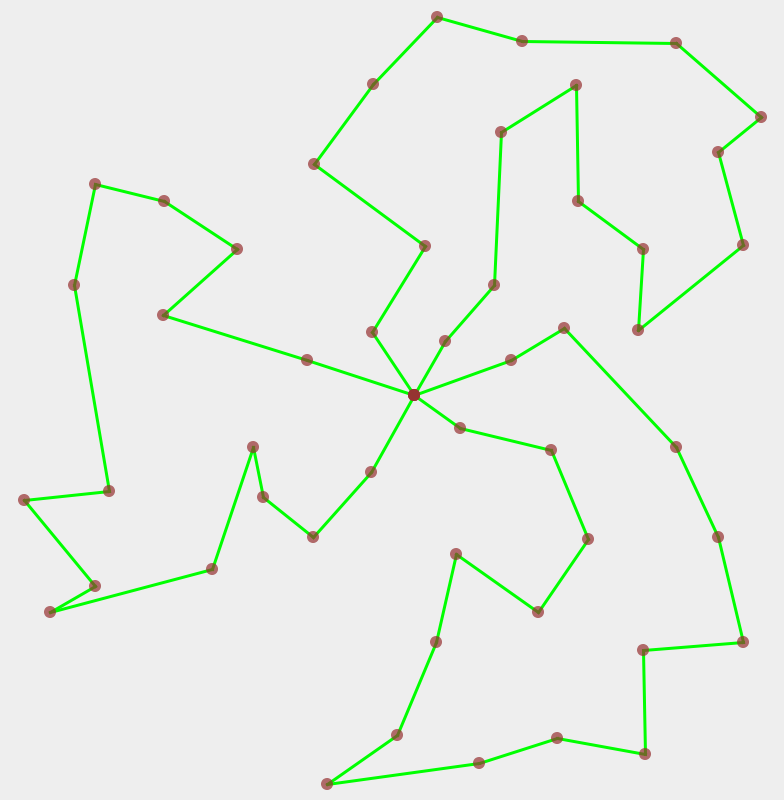
\includegraphics[width=6cm]{50_meme}
      \caption{Řešení vygenerované memetický algoritmem pro vstpu s 50 městy.}
    \label{fig:res}
\end{figure}

Byly implementovány tři algoritmy řešící problém \textit{mTSP}, respektive \textit{VRP - Vehicle Routing Problem}. Především pro menší vstupy algoritmy dosahují velmi dobrých výsledků
blízkých globálnímu optimu. Příkladem je řešení nalezené memetickým algoritmem pro 50 měst (obrázek \ref{fig:res}). Memetický algoritmus kombinující operátor křížení \textit{ordered crossover} a \textit{2-opt} lokální prohledávání je také průměrně nejlepším algoritmem při uvedené konfiguraci experimentů.
Další výzkum by se mohl věnovat optimálnějšímu určení parametrů algoritmů - ty mohou být určeny například evolučním algoritmem.

\begin{figure*}[ht]
  \centering
    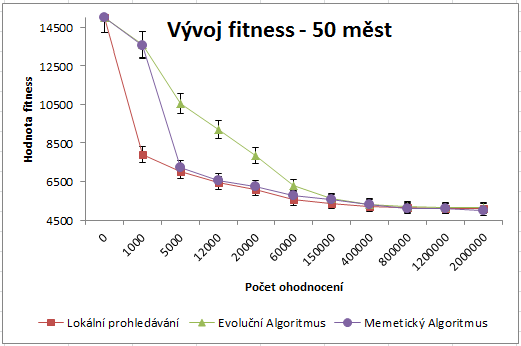
\includegraphics{results_50M}
      \caption{Výsledky algoritmů pro 50 měst}
    \label{fig:r50m}
\end{figure*}

\begin{figure*}[ht]
  \centering
    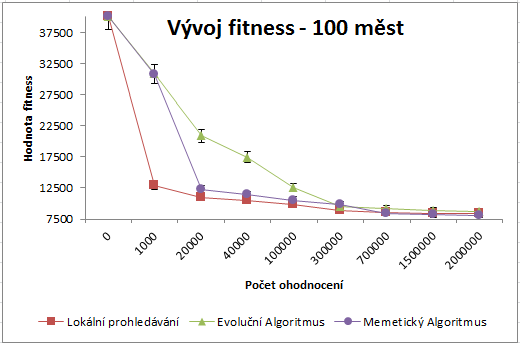
\includegraphics{results_100M}
      \caption{Výsledky algoritmů pro 100 měst}
    \label{fig:r100m}
\end{figure*}

\begin{figure*}[ht]
  \centering
    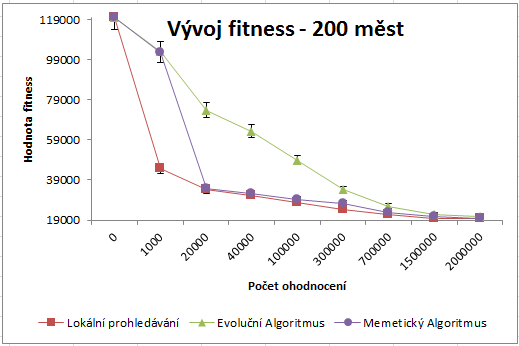
\includegraphics{results_200M}
      \caption{Výsledky algoritmů pro 200 měst}
    \label{fig:r200m}
\end{figure*}

\end{document}